\documentclass[12pt,a4paper]{report}
\usepackage[spanish,mexico]{babel} 
\usepackage[utf8]{inputenc}
\usepackage{setspace}
\usepackage[top=2.4cm, bottom=2.7cm, left=3.3cm, right=2.0cm]{geometry}   % with the script is lower the text, with kile it put +o- 1 cm above, check when pinted in the school
%\usepackage[square, comma, sort&compress]{natbib}
\usepackage{makeidx}
\setcounter{secnumdepth}{3}
\setcounter{tocdepth}{3} 		
\usepackage{url}
\usepackage{subfig}  % para usar la función subfigura
\usepackage{epsfig}  % para trabajar con figs eps 
\usepackage{multirow}
\usepackage{bigstrut}
\usepackage{booktabs}
\usepackage{rotating} 				% for vertical text in tables with  \begin{sideways}Paper\end{sideways} &\begin{sideways}Static\end{sideways} \\
\usepackage{algorithm}
%\usepackage[numbered]{algo}
%\usepackage[printonlyused,withpage]{acronym}
\usepackage{hyphenat} 			%hyphenation of compound words
\usepackage{array} 			% to increse space between rows in tables using \setlength{\extrarowheight}{1.5pt}
%\usepackage{multicol}
\usepackage{pdflscape} 			% for landscape some pages
\usepackage{textcomp} 			% for the +- sign \textpm
\usepackage{acronym}
\usepackage{graphicx}
\usepackage{pdfpages}
\usepackage{amsmath}



\graphicspath{ {images/} }

\makeindex

\begin{document}

    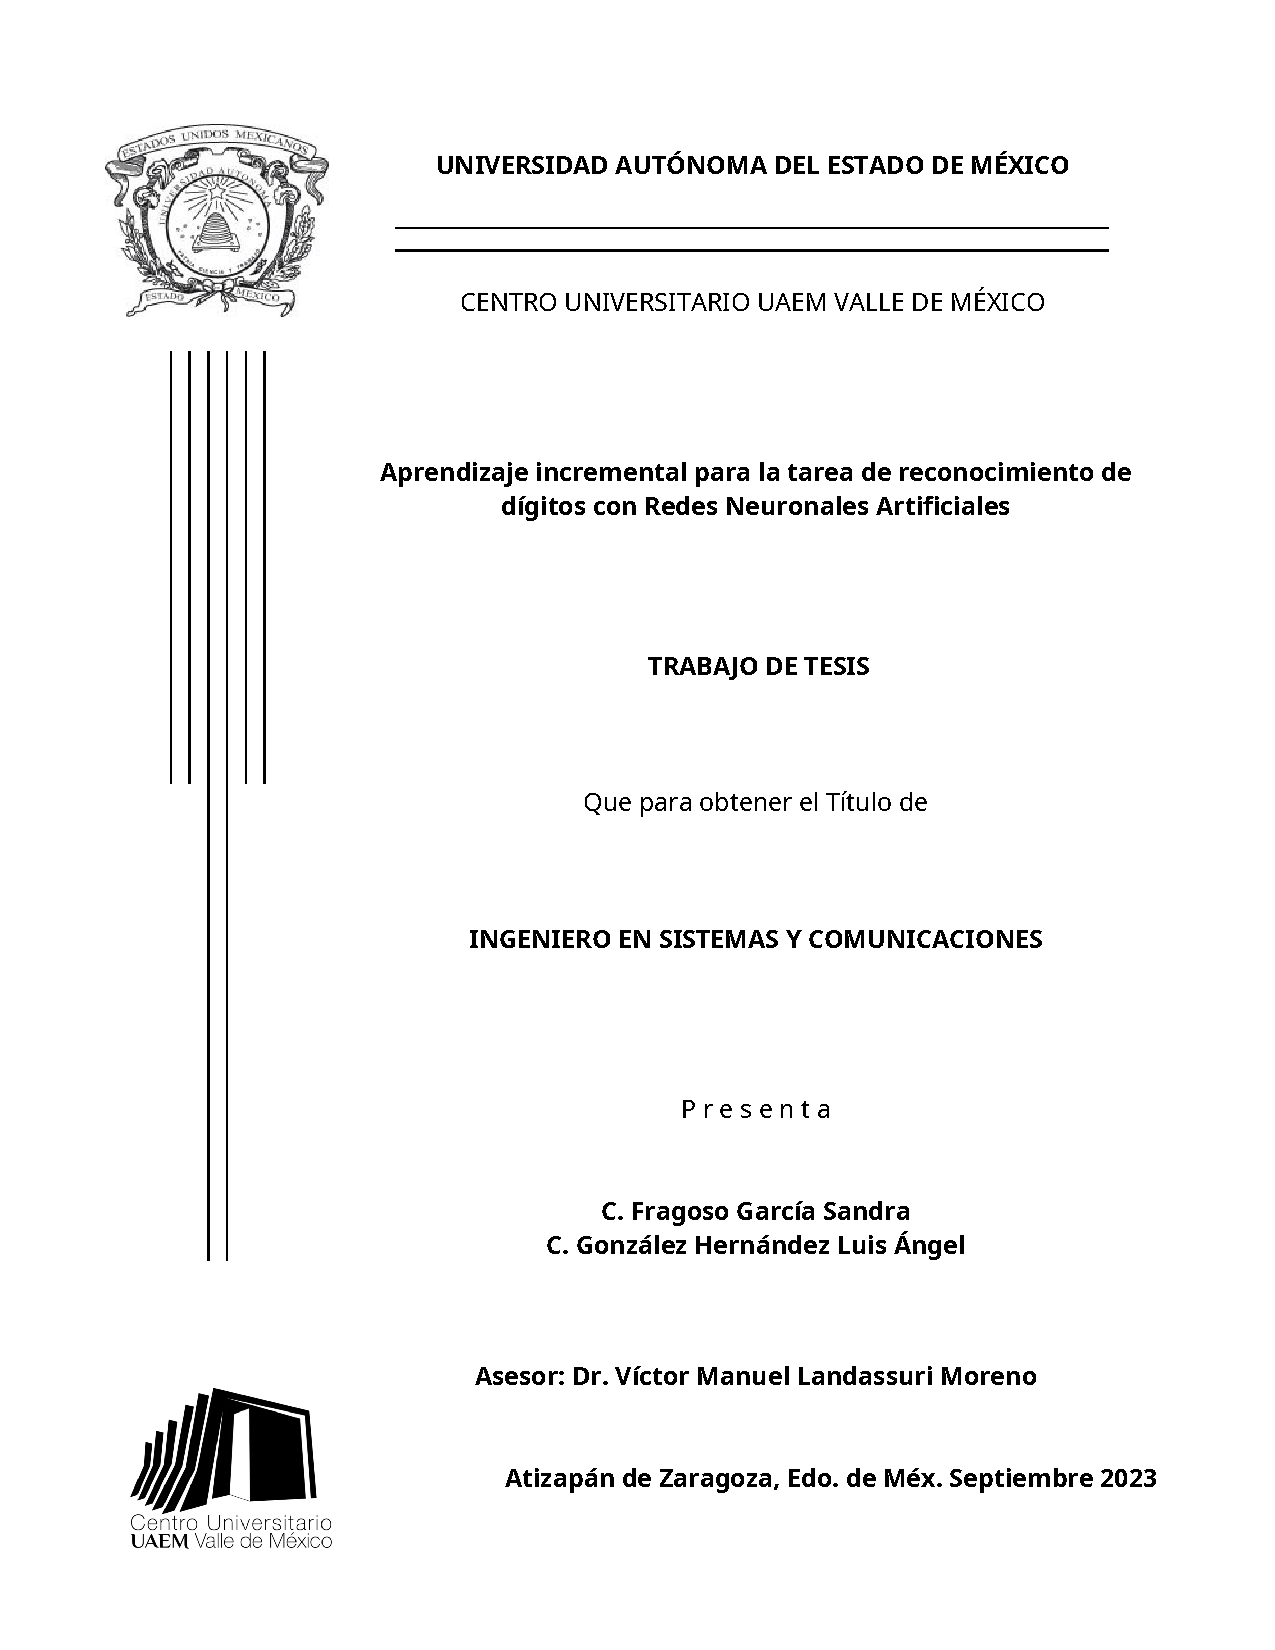
\includepdf{textFiles/portada}
    \pagenumbering{roman}
    \newpage
    \thispagestyle{empty}
    % Empty page


    % put double spacing
    \doublespacing

    \thispagestyle{empty}
    %1-2 pages
    \begin{abstract}

        El aprendizaje incremental es un área de la Inteligencia Artificial la cual permite agregar nuevo conocimiento 
        a un modelo (e.g. Redes Neuronales Artificiales) sin la necesidad de entrenar el modelo con toda la información 
        histórica de la tarea en cuestión \cite{bullinaria2009}. En el presente trabajo de investigación se ocupará el modelo de Redes 
        Neuronales Artificiales enfocada en la clasificación de dígitos escritos a mano usando el algoritmo de 
        entrenamiento de backpropagation, con redes Multi capa Perceptron y duplicación de pesos múltiples 
        simulando memoria a corto y largo plazo para mejorar los resultados presentados en \cite{bullinaria2009}.\\

    \end{abstract}

    \newpage
    \thispagestyle{empty}
    % Empty page

    % dedication
    \newpage
    \thispagestyle{empty}

    %  \addvspace{3in}
    \vspace*{2in}


    \noindent \hspace{2in} Dedicatoria 

    \newpage
    \thispagestyle{empty}
    % Empty page
    ~

    \chapter*{Agradecimientos}
    \thispagestyle{empty}


    Sus agradecimientos

    \tableofcontents

    \listoffigures

    \listoftables

    % \listofalgorithms


    \newpage
    \thispagestyle{empty}
    % Empty page
    ~

    % A c r o n y m s
    \chapter*{Lista de Acronimos}


%%%%%%%%%%%%%%%%%%%%%%%%%%%%%%%%%%%%%%%%%%%%%%%%%%%%%%%%%%%%%%%%%%%%%%%%%%%%%%%%%%%%%%%%%%%%%%%%%%%%%%%%%%%%%%%%%%%%%%%%%%%%%%%%%
% Rules for this pacage
% \ac{ acronym } 	put it, put full acronym if it is the first time
% \acresetall 		flushed the memory of macro \ac, so it will print the full acroym the first time any of them is called
% \acf{} 		Full name is printed, and the acronym is in brackets
% \acs{}		short version
% \acl{} 		expanded acronym without even mentioning the acronym

% \acp			Works in the same way as \ac, but makes the short and/or long forms into plurals.
% \acfp			Works in the same way as \acf, but makes the short and long forms into plurals.
% \acsp			Works in the same way as \acs, but makes the short form into a plural.
% \aclp			Works in the same way as \acl, but makes the long form into a plural.
% \acfi			Prints the Full Name acronym (\acl) in italics and the abbreviated form (\acs) in upshaped form.
% \acused		Marks an acronym as used, as if it had been called with \ac, but without
% 			printing anything. This means that in the future only the short form of the
% 			acronym will be printed.
% 
% \acsu			Prints the short form of the acronym and marks it as used.
% \aclu			Prints the long form of the acronym and marks it as used. Example: \acl{lox}/\acl{lh2} (\acsu{lox}/\acsu{lh2})
% \...*			The following commands do the same as their unstarred forms, except that the
% 			acronym will not be marked as used. If you work with the ’onlyused’ option then
% 			macros which have only been used with starred commands will not show up.
% 			\ac*, \acs*, \acl*, \acf*, \acp*, \acsp*, \aclp*, \acfp*, \acfi*, \acsu* and
% 			\aclu*.
%
% For more information see the manual: /media/dat/LIBROS/Latex/acronyms/acronym.pdf
%%%%%%%%%%%%%%%%%%%%%%%%%%%%%%%%%%%%%%%%%%%%%%%%%%%%%%%%%%%%%%%%%%%%%%%%%%%%%%%%%%%%%%%%%%%%%%%%%%%%%%%%%%%%%%%%%%%%%%%%%%%%%%%%%




% Previous version

%\begin{table}[b]
  	%\caption{Multiple-step, closed-loop or iterate forecasting}
%		\centering
%			\begin{tabular}{llll}
				%\hline\noalign{\smallskip}
				%${Forecast}$ & $Inputs$ \\
				%\noalign{\smallskip}
				%\hline
				%\noalign{\smallskip}
%& MSP & & Multi step prediction \\
%& SSP & & Single step prediciton \\ 
				
				%\hline
%			\end{tabular}\\
%			\vspace{-2mm}
%		\label{MultipleForecasting}
%	\end{table}

    %\newpage

    \pagenumbering{arabic}

    % put double spacing
    \doublespacing



    % Each one is a chapter 
    \section{Introduccion}

El aprendizaje incremental es un método el cual a sido implementado en el área de la inteligencia artificial, ya que al realizar tareas especificas de dicha rama nos 
ayuda a optimizarla para que el algoritmo sea más eficiente.
Cualquier tipo de aprendizaje puede ser considerado aprendizaje incremental si el problema a resolver tiene un entrenamiento simple, adem\'as este tipo de algoritmo es conocido como \textit{algoritmo lineal sin memoria},
en la mayor\'ia de los casos este tipo de aprendizaje es el preferido o favorito por los desarrolladores \cite{GiraudCarrier2000}.

Las redes neuronales artificiales (RNAs) son procesos matem\'aticos los cuales son utilizados en el \'area de Machine Learning para 
la resoluci\'on de problemas no lineales, estos deben de pasar por una funci\'on de activaci\'on la cual es una multiplicaci\'on 
entre lo valores otrogados, al ser procesados por las capas que contenga la neurona, obtendremos un valor distinto al de entrada.

Adem\'as son una distribuci\'on muy conocida de parte del Machine Learning, de otra manera es el poder que tienen las computadoras para una buena estructura distribuida en paralelo y una buena habilidad de aprendizaje, 
este modelo computacional se define por medio de las neuronas biologicas las que son encargadas de que el ser humano pueda aprender o distinguir de distintos aspectos, este tipo de 
metodo es motivado para poder obtener la meta de un buen aprendizaje de maquina \cite{liu2015}.

Un factor importante para esta rama es la perdida de memoria, este es un problema biol\'ogico, el cual tanto afecta a los humanos como a las maquinas, es por eso que se han elaborado distintos
experimentos para poder convatir esta problematica.
Uno de  estos es el caso de John Bullinaria, quien maneja la arquitectura de doble peso, ya que en su experimento da a notar que mejora la utilizaci\'on del aprendizaje incremental, esto se logro 
con sistemas existentes como lo es Learn++.

Cabe mencionar que el experimento realizado fue un problema de generalizaci\'on m\'as comunes, pero se necesitan m\'as evidencias 
de que usando esta metodolog\'ia sirve para utilizarlo no solamente en tareas generalizadas, adem\'as se espera un mejor rendimiento \cite{Bullinaria2009}.  \\


\section{Planeamiento}

    Indicar de forma general como es el funcionamiento de las redes neuronales en el uso general, como es que se produce la falta de memoria en 
    estos modelos de predicciones. Poner en pr\'actica los modelos de experimentación de John Bullinaria para comprobarlos con
    problematicas m\'as robustas y optimizarlo para que sea un m\'etodo eficiente.

    \newpage
    \thispagestyle{empty}
    % Empty page
    \section{Planeamiento}

    Las Redes Neuronales Artificiales tienen la habilidad de poderse aprender una tarea, 
    y poder hacer o resolver tareas de predicción o clasificación básicamente. En este 
    sentido, con algoritmos de aprendizaje como el Backpropagation, permite ajustar los 
    pesos de una RNA para que esta pueda empezar a resolver una tarea particular.  No 
    obstante, muchas de las tareas que se resuelven en la vida diaria, van generando mas 
    información con el tiempo, por ejemplo, el comportamiento de un una serie financiera, 
    o bien la predicción del clima en una determinada región. Así,  se tiene el aprendizaje 
    incremental, siendo un método poco explorado,  enfocado en poder aprender nueva información del 
    problema, sin tener que volver a entrenar todo el modelo con la información anterior, y la 
    nueva que acaba de llegar, esto es, en los modelos actuales de aprendizaje máquina, si se usa 
    un conjunto de datos para entrenar un modelo en especifico, dicho modelo es funcional para 
    dicho conjunto de datos y la información que ello representa. Sin embargo, si es necesario 
    incorporar nueva información al modelo, es necesario recolectar dicha información nueva, 
    agregarla a la que se tenia anteriormente, y volver a entrenar todo el modelo para que \'este 
    pueda incorporar la nueva información.

    De esta forma, una red ya entrenada con un primer conjunto de datos $d_{1}$ se desea entrenar 
    con un nuevo conjunto de datos del mismo problema $d_{2}$, al entrenar la red con $d_{2}$ se 
    perderá en conocimiento aprendido por $d_{1}$.  Si no se desea utilizar un modelo de aprendizaje 
    incremental, se tendría que juntar el conjunto $d_{1}$ y $d_{2}$ en un solo conjunto y volver a 
    entrenar la RAN para así poder incorporar el nuevo conocimiento ($d_{2}$) a la RNA. Si se desea 
    utilizar el método de aprendizaje incremental, se puede entrenar en un primer moemnto a la red 
    con el conjunto $d_{1}$, posteriormente con $d_{2}$ teniendo poca perdida de información de $d_{1}$. 
    Si más adelante llega mas información del problema ($d_{3}$) que se desee incorporar a la base 
    de conocimientos de la RNA, entonces solo habrá que entrenar la RNA con $d_{3}$ usando el modelo 
    incremental para tener una p\'erdida mínima de información de $d_{1}$ y $d_{2}$. 

    De esta forma, el presente trabajo tomar\'a como base la investigación de \cite{bullinaria2009}, 
    en donde utiliza una configuración de pesos dobles (a una RNA se duplican todos sus pesos), 
    donde a una capa de pesos duplicados se enlaza con una tasa de aprendizaje alta, para simular un 
    rápido aprendizaje, y por ende simular lo que sería memoria a corto plazo. En su contraparte, 
    la segunda capa de pesos duplicados, se enlaza con una tasa de aprendizaje baja para aprender 
    lentamente un problema, simulando la memoria a largo plazo.  Es decir, al momento de aprender una 
    tarea nueva,  una capa de pesos aprenderá muy rápido la nueva tarea (tasa alta de aprendizaje) y 
    por ende olvidará más rápidamente los datos ya aprendidos anteriormente, por otro lado, la segunda 
    capa de pesos duplicados, aprenderá muy lentamente los nuevos datos que llegan, y por ende olvidando 
    poco la información que anteriormente se aprendió.  Considerando ello y también que la 
    RNA trabaja en conjunto con ambas capas de pesos duplicados, se pondera la salida de la RNA para 
    que pueda contemplar la información nueva que se acaba de agregar a la RNA, en ambas capas, así como 
    la información que se acaba de olvidar de ambas capas de pesos.

    El problema principal del aprendizaje incremental mostrado en \cite{bullinaria2009}, es que entre 
    más conjuntos de datos nuevos que lleguen, mas se olvidaran los primeros conjuntos que se aprendieron, 
    lo cual no es tan útil si se contempla que en el futuro de una RNA podrán existir 10 o 20 etapas de 
    entrenamiento incremental con nuevos conjuntos de datos que se vayan recolectando.

    Por ello es indispensable poder explorar nuevas configuraciones de RNAs que permitan mejorar los 
    métodos actuales para permitir una menor cantidad de olvido conforme llegue nueva información al 
    modelo. Donde al igual que en trabajos anteriores,  el presente trabajo se basará en conceptos de 
    memoria a corto y largo plazo, y en lugar de hacer una copia de los pesos actuales y tener dos 
    tasas de aprendizaje, una rápida para simular la memoria a corto plazo, y otra tasa de aprendizaje 
    para simular la memoria a largo plazo, se explorará por hacer mas copias de los pesos, teniendo más 
    tasas de aprendizaje que operen en cada una de dichas copias.
    
    \section{Objetivos}
    Diseñar una red neuronal artificial para aprendizaje incremental basada en el principio de la memoria a corto y largo plazo, buscando usar más de dos capas de pesos duplicados para el reconocimiento de dígitos, y con una menor p\'erdida de información de trabajos previos.
    \subsection{Objetivos Particulares}
        \begin{enumerate}
            \item Implementar el algoritmo mostrado en \cite{bullinaria2009} para el reconocimiento de dígitos con aprendizaje a corto y largo plazo con los parámetros que ahí se indican.
            \item Obtener el conjunto de datos de Optical Digits, limpiar los datos y prepararlos según lo indicado con \cite{bullinaria2009}.
            \item Separar el conjunto de entrenamiento y de prueba de acuerdo a lo que se explica en el artículo de Bullinaria y probar el primer código implementado en miras de comprobar los resultados previamente mostrados en \cite{bullinaria2009}.
            \item Tomar como base el algoritmo implementado, y extenderlo para permitir mas de dos pesos duplicados, aplicando el conjunto de datos previamente mostrado.
            \item Comparar ambas implementaciones en busca de una reducción significativa de las tasas de aprendizaje con respecto a trabajos previos en la literatura.
        \end{enumerate}
    \chapter{Preguntas de investigación}

\begin{enumerate}
  \item ¿Existen trabajos más recientes sobre aprendizaje incremental?
  \item La memoria a corto y largo plazo, representa dos extremos, pero ¿será posible subdividir más esa clasificación, para que más puntos intermedios puedan mejorar la memoria a corto y largo plazo, al mismo tiempo que el rendimiento en el aprendizaje incremental?
  \item ¿El uso del aprendizaje incremental va a hacer que el tiempo de entrenamiento sea  m\'as r\'apido o al contrario?
\end{enumerate}
    \section{Justificaci\'on}

    Las redes neuronales permite el aprendizaje automático y la resoluci\'on 
    de distintos problemas,  pero como se comentó anteriormente,  las técnicas 
    de aprendizaje máquina, tiene una deficiencia que es al momento de aumentar 
    los nuevos bloques de datos que lelguan para aprender,  se obtiene un deteriro 
    en el rendimiento de aprendizaje de información y olvido de la información anterior
    \cite{bullinaria2009}.   (REFIVEN COMO VOY PONEINDO LA REDACCIÓN DE LO QNTERIOR, Y 
    CO NELLO TRATEN DE CAMBIAR LO QUE VIENE PARA QUE LE MOJOREN EL ESTILO, DE AQUÍ EN 
    ADELANTE SOLO LES HARE OBSERVACIONES EN ESPERA QUE USTEDES MEJOREN EN GENERAR LA 
    REDACCIÓN) Los resultados que se han obtenido no funcionan a la perfección, la 
    memoria a corto plazo olvida poco pero va olvidando, y lo ideal sería que no 
    olvidara. Biológicamente los humanos pueden aprender nuevas tareas, o información 
    nueva de un problema, y no olvida de forma siginficativa lo que anteriormente 
    aprendio, no obstante eso no pasa actualemnte co loas RNA y en general con 
    cualquier algoritmo de aprendizaje máquina, . En otro sentido los humanos 
    ya tenesmo cierta configuración en el cerebro que nos permite aprender como 
    lo hacemos actualmente,  y se peude afirmar que por elmomento no hay ningun 
    procedimiento (quirurjico o no) que permita modificar la estructura del cerebro 
    para aprender mas y olvidar menos. 

    No obstante,  computacionalmente nada puede impedir que se experimente con más 
    configuraciones y llegar al punto en donde toda la información que ingrese a un 
    modelo (e.g. RNAs) se acumule y si no hay problema de almacenamiento que se siga 
    acumulando y que no olvide, eso podría ser bueno en diversas situaciones.

    Desde el punto de vista computacional, si llega nueva información y no se ocupa aprendizaje 
    incremental, ello implicara volver a entrenar todo el sistema con la información anterior y 
    la actual (e.g. $d_{1}$ y $d_{2}$) y considerando que una de las desventajas que tienen la 
    RNAs es que el entremainento es un cuello de botella, siendo este donde se llevá la mayor 
    parte de cómputo y por consiguenote de energía. Ello implica que volver a entranar con todo 
    la infomación acumulada, gastará más energía y tiempo que si solo se entrana con la nueva 
    información que llega al modelo. En su contraparte,  existe una gran variedad de herramientas 
    las cuales permiten codificar una red neuronal artificial con librerias ya preexistente, por 
    el momento se expondrán solo 2 empresas, siendo estas las más importantes: Microsoft y Google. 
    La primera cuenta con la plataforma de Azure que nos renta una maquina virtual donde se puede 
    programar en Python.  Por el contrario, Google cuenta con Google Colab que igual nos brinda 
    una maquina virtual para realizar experimentos de Maching Learning, la \'unica diferencia 
    contra Azure es que dicha herramienta es gratuita, una similitud que tienen es que en las 
    dos se puede programar en el mismo lenguaje.

    Como se observa ambas herramientas permiten la programaci\'on en Pyhton y esto se debe a que 
    dicho lenguaje es una herramienta de software libre que no requiere licencia, es relativamente 
    fácil poder depurar un código y permite acelerar más el desarrollo de aplicaciones,  a diferencia 
    de otros lenguajes más estructurados como C o Java, adem\'as tiene m\'as librerías para el 
    desarrollo de Maching Learning e.g TensorFlow, Numpi, entre otras. \\

    TensorFlow es una librería de Python que permite construir y entrenar redes neuronales para 
    detectar patrones y razonamientos usados por los humanos, en la presente investigaci\'on se 
    usar\'a dado a que favorece la creaci\'on de una RNA, permite la elaboraci\'on de cualquier 
    tipo de algoritmo de Machine Learning, cabe mencionar que también se puede usar para Deep Learning, 
    facilita la adquisici\'on de datos modelos de capacitaci\'on, predicciones y refinamiento de 
    resultados, esta disponible para el uso en computadores personales, pero es recomendado 
    usarlo en su propio editor en la nube que es Colab. \\ 

    Keras (MISMO COMENTARIO QUE LES PONGO DE TENSORFLOW)es un framework de alto nivel para 
    el aprendizaje, escrito en Python y capaz de correr sobre los frameworks TensorFlow. Fue 
    desarrollado con el objeto de facilitar un proceso de experimentación rápida. Diseñado 
    para construir por bloques la arquitectura de cada red neuronal, incluyendo redes 
    convolucionales y modelos recurrentes, que son las que permiten, junto a los bloques 
    "más tradicionales", entrenar aprendizaje profundo.
    \section{Delimitación}
\label{sec:delimitation}
	
	
    En la presente investigación solamente se utilizará redes neuronales del tipo perceptr\'on multicapa,  donde 
    cabe mencionar que este no es el único tipo de red que existe, i.e., también se tiene Redes Neuronales Convolucionales (RNC), Redes Neuronales Recurrentes (RNR) o bien Redes de Base Radial (RBR) \cite{royo2021}. Así mismo, no se abordará el uso de técnicas d eoptimiación como lo son los algoritmos genéticos, y unicamente se limitará a explorar la mejora en rendimiento al tener más de dos capas duplocadas de pesos en la red con aprendizaje incremental.  Así mismo, no se abordarán modelos como las redes profundas u otro conjunto de datos y se limitará el trabajo a lo antes mencionado.



    
    \chapter{Revisión de la Literatura}
  \section{Redes Neuronales Artificiales}
  
    Las redes neuronales artificiales (RNA) son modelos computacionales de la Inteligencia Artificial los cuales contienen simples unidades de procesamientos llamadas neuronas.  Ellas se inspiran en el cerebro humano, tomando como base la conectividad entre neuronas y el aprendizaje que pueden tener.  Un perceptron o neurona (artificial) solamente resuelve problemas lineales y tiene la siguiente forma:
    
    \begin{figure}[H]
      \centering
      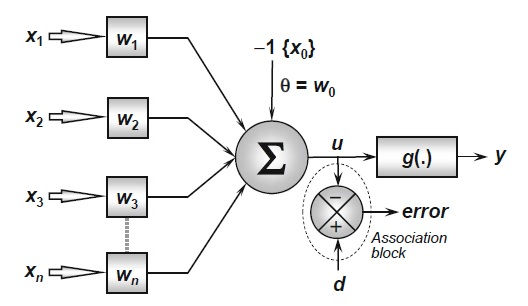
\includegraphics[width=\columnwidth]{ANN.jpg}
      \caption{Red Neuronal Artificial B\'asica}
      \label{fig:fig1}
    \end{figure}

    Donde $\Sigma$ es la representación matemática de la neurona.,  $x_1$, $x_2$,  \dots  ,$x_n$ son las variables de entrada a la red.  $w_1$,$w_2$,  \dots , $w_n$ son los pesos con los cuales se van a podnerar las entradas, es decir multiplicar cuando la información entra en la neurona. Posterior a multiplicar el peso por la entrada correspondiente,  se suman todos esos valores $w_1$$x_1$ + $w_2$$x_2$ + $w_3$$x_3$.


    \section{Metodología}
    El primer paso a realizar en esta investigación es recrear el código mostrado en \cite{bullinaria2009}, donde se describe la implementación de una red  neuronal multicapa usando el algoritmo de entrenamiento backpropagation en el lenguaje de programación Python.  Para esto se utilizará el conjunto de datos de Optical Digits,  en donde se tendrá que preprocesar los datos, para eliminar registros inválidos. 

    Posteriormente se implementará una nueva versión del código en donde se experimentará con mas de dos capas de pesos duplicados para mejorar la tasa de olvido de información al momento de usar el aprendizaje incremental.  Para ello se explorará incrementando gradualmente el nueron de capas (esto no lo entendi,neuronas de capas?)de pesos duplicados, hasta llegar al punto en que mas capas no generen un decremento de las tasas de olvido/error.

(REVISEN LA REDACCIÓN Y MEJORENLA DE FAVOR)
    Cuando los dos proyectos se tengan, se realizar\'a una comparación, donde se ver\'a cual de estos dos experimentos
    es más eficaz en proyectos de la vida real.
    
\section{Cronograma de Actividades}
(EL CRONOGRAMA DE ACTIVIDADES DICE JOHN BULLINARIA EN LA PARTE DE ARRIBA, ELIMINAR ESO)

    \begin{figure}[H]
        \centering
        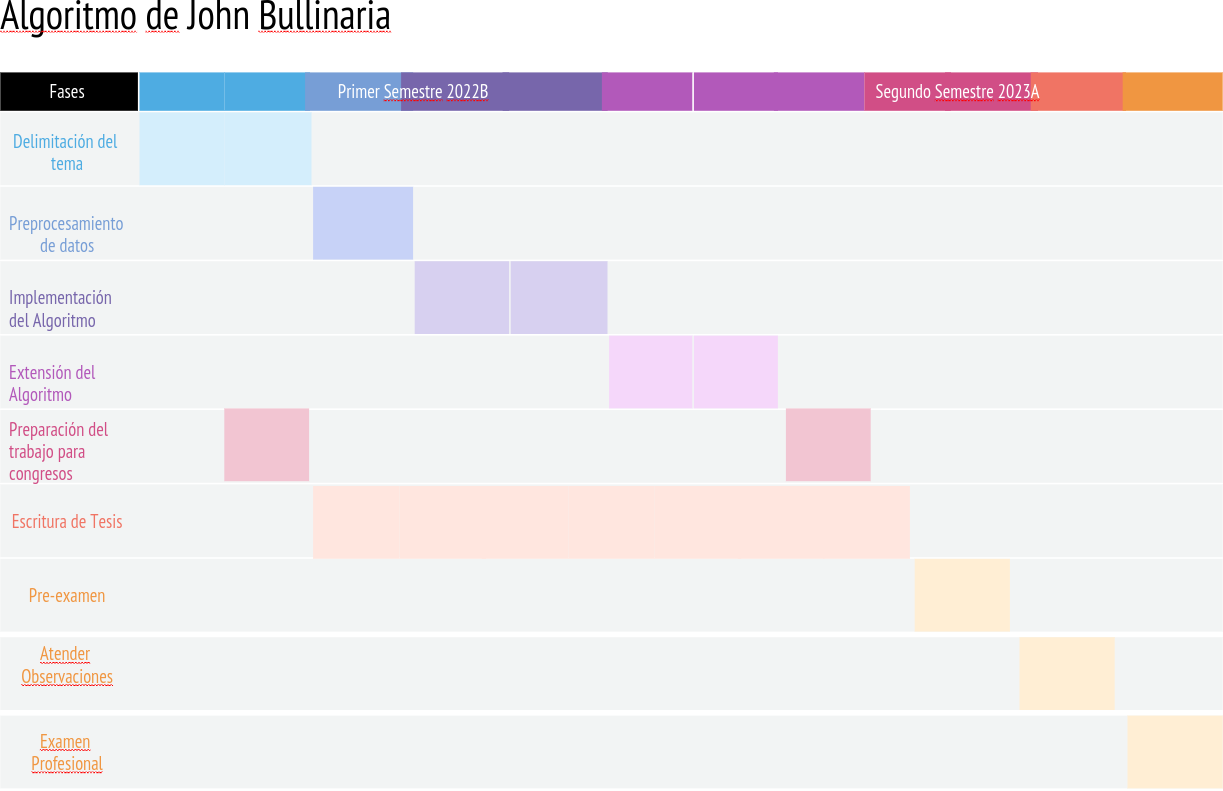
\includegraphics[width=\columnwidth]{diagramaGantt.png}
        %\caption{Elimine estoa horita, no hace falta ponerle un titulo, dado que es la únic figura en la sección}
        \label{fig:fig3}
    \end{figure}

\section{Organización del Capitulado}


	En el capitulo 2 se ver\'a lo que es el aprendizaje humano y el aprendizaje incremental con sus algoritmos, se describirán las redes neuronales artificiales.

En el capitulo 3 se implementar\'a el articulo de John A. Bullinaria, como funciona, resultado que da al pasar los datos que dice para comprobar que funciona como menciona en su art\'iculo. En el capitulo 4 se explicar\'a como se hará la modificación a su algoritmo, cuantas capas se van a poner, como se van a repartir las tazas de aprendizaje.

Posteriormente en el capitulo 5 se mostrar\'a una comparación de los resultados de ambos trabajos. En el capitulo 6 se verán las conclusiones y trabajo futuro.

    
\section{Organización del Capitulado}


	En el capitulo 2 se explicar\'a lo que son y como funcionan las redes neuronales artificiales, as\i como la función de activación que es un método que utilizan estas.
	 Se describir\'an los tipos de redes neuronales, tanto de perceptron multicapa como convolucionales, y el algoritmo backpropagation.
	 Se mencionar\'a como es el aprendizaje en humanos, que este se divide en el aprendizaje activo y el aprendizaje con comprensión
	 Y para terminar se describirá el aprendizaje incremental y su algoritmo.\\
	 
	 En el capitulo 3 se implementar\'a el algoritmo de John A. Bullinaria, se verificar\'a su funcionamiento y los resultados que da al pasar los datos que dice para comprobar que es como menciona en su art\'iculo.\\
	 En el capitulo 4 se explicar\'a como se se extendió el algoritmo base permitiendo el uso de mas de dos pesos duplicados y se aplicaran los mismos datos de entrenamiento y de prueba que al algoritmo base.\\
	 
	 Posteriormente, en el capitulo 5 con los resultados obtenidos, se mostrar\'a una comparación de los resultados de ambos trabajos para notar si hubo una reducción significativa en las tasas de aprendizaje. En el capitulo 6 se verán las conclusiones y trabajo futuro.

    %\bibliographystyle{acm}
    \bibliographystyle{ieeetr}%plain}
    \bibliography{dataset.bib}
    %\bibliography{BaseDatos2}


%\printindex
\end{document}

